
\documentclass[submit, techrep]{ipsj}
%\documentclass{ipsj}

\usepackage[dvipdfmx]{graphicx}
\usepackage{latexsym}
\usepackage{color}
\usepackage{amsmath}
\usepackage{siunitx}

\input{00_macro}

\def\Underline{\setbox0\hbox\bgroup\let\\\endUnderline}
\def\endUnderline{\vphantom{y}\egroup\smash{\underline{\box0}}\\}
\def\|{\verb |}


\setcounter{巻数}{59}
\setcounter{号数}{1}
\setcounter{page}{1}

\makeatletter
\pagestyle{empty}
\def\@oddhead{}%
\def\@evenhead{}%
\def\ps@IPSJTITLEheadings{}
\makeatother







\begin{document}


\title{距離センサアレイを用いた膝によるカーソル操作手法}



\affiliate{CS1}{筑波大学 システム情報工学研究科 \\コンピュータサイエンス専攻}
\affiliate{CS2}{筑波大学 システム情報系}


%\paffiliate{JU}{情報処理大学\\
%Johoshori University}

\author{市川 佑}{}{CS1}[yichikawa@iplab.cs.tsukuba.ac.jp]
\author{志築 文太郎}{}{CS2}[shizuki@cs.tsukuba.ac.jp]
\author{高橋 伸}{}{CS2}[shin@cs.tsukuba.ac.jp]

\begin{abstract}
本研究では,机裏に設置した距離センサアレイにより,膝の位置を認識し,カーソル操作に応用することを提案する.
膝による入力を実現することで,手といった他の入力モダリティとも組み合わせることができる可能性がある.
ユーザは机の前に座り,机の下で膝を上下左右に動かすと,カーソルを操作できる.
%これはキーボードなどの手による操作と並行して行うことができる.
机の裏に機器を設置することにより,ユーザの邪魔になりにくく,身体に装置を取り付ける必要もない.
我々は.
%距離センサアレイを製作し,
膝の位置の認識,膝の位置からカーソル座標への変換を行うシステムを実装した.
システムは簡単なキャリブレーションを行うことで,様々な体格の人に対応させることができる.
我々はシステムをカーソル操作に適用し実験を行い,膝の操作性やユーザの疲労感,上下左右方向への膝の運動の難易を調査した.
%さらに,膝による操作の応用例として,一人称視点ゲームへの適用を提案する.
\end{abstract}






\maketitle

%1
\section{はじめに}
%様々なペダルの操作に代表されるように,我々は日常的に足による操作を行っている.
%しかし,パーソナルコンピュータやスマートフォンを操作する際,我々は手を中心に操作を行い,足に操作が割り当てられることはなく,ほとんど動かすことがない.
一般に椅子に座り机上で作業をする場合、手を用いることが多い.例えば,コンピュータを用いる作業では両手をマウスやキーボードの操作に充てることが多い.一方で足は操作が割り当てられることはなく,ほとんど動かすことがない.操作を足に割り当てることができれば、手による操作を中断することなく他の入力を行うことができ、さらに手と足を組み合わせた操作の拡張も可能となる。\par
足による操作を用いたコンピュータ向けインタフェースの研究は,
%1960 年代から存在している\cite{1698228}が,現在は手による操作が中心である.
昔から行われており,先行研究には膝でレバーを操作する方法\cite{1698228}、机に取り付けた装置を足で動かす方法\cite{Pearson:1986:MMD:22627.22392, Pearson:1988:EEP:57167.57169}や,足の位置によって摩擦力を変えることができる機構を取り付けた靴\cite{Horodniczy:2017:FHE:3025453.3025625}を用いる方法がある.
これらは身体の一部に装置を取り付けるあるいは大型な装置を用いるものであるため,ユーザの衣服などに制限が生じる,装置を持ち運ぶことができないといった制約がある.\par
%しかし,手がふさがった状態における機器の操作\cite{Fan:2017:ESF:3123021.3123043}など,足によるインタラクションの研究は関心が高まっている.\par
これらの問題から、我々は膝をコンピュータの入力に用いることを提案する。膝による入力を実現するため、机の下に取り付けることにより,膝の位置を認識する距離センサアレイを開発した.
これにより,特別な装置を足に取り付けることなく,かつ小型な装置で,足を用いて入力することが可能になる.
膝による入力を実現することで,手といった他の入力モダリティとも組み合わせることができる可能性がある.
本研究ではその第一歩として,認識した膝の位置をマウスカーソルの操作に適用し,膝単体での特徴を調査する.


%膝を使う理由は 2 点ある.
%1点目に,膝は足先と比べてより自由な操作が行える可能性がある.2点目に,膝と足による操作の組み合わせによりさらにインタラクションが拡張できる可能性がある.

\section{関連研究}
\subsection{足を用いたジェスチャ入力}
足による入力に焦点を当てている研究では,まず足のジェスチャを用いるものが挙げられる.
まず,屋外でスマートフォンなどを操作するときに荷物を持っている,手が汚れているというすぐに手を用いることができない状況を想定した研究を挙げる.
Fanら\cite{Fan:2017:ESF:3123021.3123043}は,足のジェスチャによりモバイル端末を操作することに対する実証研究を行った.
荷物を持ったまま,ユーザ定義の足のジェスチャを用いて操作する方法と,荷物を降ろして手で端末を持ち操作する方法を比較したところ,前者の方が70\%高速な操作が可能であるという結果となった.
HanらのKick\cite{Han:2011:KIU:2037373.2037379}では,蹴り出すジェスチャを端末操作に用いるために,ユーザがキックの方向と速度をどの程度操作できるかを調査した.\par
本研究は,屋内での利用のみを想定した環境設置型の装置を用いるという点と,ラップトップコンピュータやデスクトップコンピュータへの利用を想定しているという点から,インタラクションの目的は異なる.\par
%また,屋内環境を想定して装置を設置することでインタラクションを実現した例として,AugstenらによるMultitoe\cite{Augsten:2010:MHI:1866029.1866064}では,巨大なタッチパネルを床面に設置し,複数の足の認識や足の重心位置の認識した.
%これにより,床面に表示されたメニューやキーボードを足で操作することを提案した.
%この研究では立った状態を想定しているが,本研究では,デスクトップ上での作業中という限定された環境におけるインタラクション手法の提案を目指す.


\subsection{机上での作業における足を用いた入力}
机上におけるコンピュータの操作に足を用いた入力手法を調査,提案した研究例を挙げる.
%Saundersら\cite{Saunders:2016:TFI:2901790.2901815}は,立った状態でのデスクトップアプリケーションの制御に足を用いた.
Pearsonら\cite{Pearson:1986:MMD:22627.22392, Pearson:1988:EEP:57167.57169}は「モル」という装置を開発し,ポインタの操作などに手の代わりに足を使用する方法を調査した.モルを用いた場合でも,訓練によって小さなターゲットを選択することが可能になることを示した.
Horodniczyら\cite{Horodniczy:2017:FHE:3025453.3025625}は,ユーザの靴に可変摩擦式の装置を取り付け,足によるカーソル操作の補助装置として用いた.靴底には低摩擦材と高摩擦材の2つを取り付け,高摩擦材の接地圧力をステッピングモータで制御する.足の位置をカメラにより取得し,ターゲットに近づくにつれ圧力を高めることで,足によるカーソル操作の補助を行う.
Vellosoら\cite{velloso:hal-01599657}は,座っている状態における机の下の足の動きの特徴を調査した.机の下に配置したカメラから,片方の足のつま先をマウス操作に割り当て,1次元と2次元におけるポインティング作業により,パフォーマンスのテストを行っている.
これらの研究では,大型の装置を用いているために持ち運びや設置が困難であったり,靴に装置を取り付けるためにユーザに身体上の制約を強いてしまう.
本研究では小型で設置が簡単かつ足に装置を取り付けないアプローチをとることで,問題の解決を図る.
また,本研究は足先でなく膝に焦点を当てることで,既存手法との組み合わせによってさらなるインタラクションの拡張を図ることも可能である.\par
足と他の入力モダリティとの組み合わせを行った研究としては,次のようなものが存在する.
G\"{o}belら\cite{Gobel:2013:GFI:2468356.2479610}が提案する手法では視線認識と足の動きを組み合わせ,視線位置におけるパンとズームの操作を足によるペダル操作で行うことを提案した.
Rajanna\cite{Rajanna:2016:GFI:2876456.2876462}は,視線によるポインティングと足によるクリックコマンドで構成されるシステムを構築した.\par
本研究では膝による入力操作を行うことで,最終的に手による入力との組み合わせを目指す.また膝を用いることで、手だけでなく足による入力とも組み合わせることができる可能性がある。

\subsection{膝を用いたコンピュータへの入力}
膝に関する研究の中で,コンピュータへの入力を想定したものは少ない.
Englishら\cite{1698228}は,テキスト選択において,いくつかの装置を用いたときの操作時間を調査した.装置の中には膝で動かすものも含まれている.
調査の結果,膝による操作は最も短い時間でテキストを選択できることができることがわかった.
この研究では,机の下に取り付けた装置のレバーを膝で動かすことで入力を行った.しかし、ユーザは座る位置をレバーに合わせなければならず、またレバーを動かすために力をかける必要がある.\par
%この装置は調査を行うために作られた原始的なものであった.
本研究では距離センサを用いており,ユーザが膝を距離センサアレイの範囲内に位置させ、キャリブレーションを行えば、比較的自由な位置で操作することができる.さらにユーザは膝で装置を動かす必要がないので、疲労感を少なくすることができると考える.

\section{膝によるカーソル操作の設計}
椅子に座った状態では膝を左右に傾けることは容易に行うことができるが、マウスやタッチパッドの操作と異なり,前方や後方に動かすことは困難である.
そのため,本研究で想定する膝の移動は,膝を左右に傾けることによる左右方向と,かかとを浮かせたり床につけたりすることによる上下方向の移動である.
\refImg{knee_howto}は,ユーザが膝をどのように動かすかを表したイメージである.
\img{tb}{1}{sousa_overview.pdf}{カーソルの位置に対するユーザの膝のイメージ}{knee_howto}

マウスカーソルを左右に移動するときには,膝を左右に傾ける.
上方向に移動するときは,かかとを浮かせて膝を机に近づける.
逆に下方向に移動するときは,足を手前に引き,そのときに浮いたかかとを床に近づけることで,膝を机から遠ざける.
足が完全に地面についているときにカーソルが画面の中心にあるため,ユーザは比較的楽な姿勢で操作することができる.

\section{プロトタイプシステムの実装}
プロトタイプシステムは,三角法を用いた光学式距離センサ 10 個を一列に並べた距離センサアレイ,マイクロコンピュータ,およびPCからなるハードウェアと,センサから距離データを取得し,膝の位置の認識,キャリブレーションの記録,カーソル座標への変換を行うソフトウェアからなる.システムの処理の流れを\refImg{system_overall}に示す.\par
まず距離センサアレイからマイクロコンピュータが距離データを取得する.マイクロコンピュータ上のプログラムは,\iic 通信により距離センサから膝との距離を取得する.これを10個の距離センサ全てについてそれぞれ行う.さらに,計測された10個の距離を1フレームにまとめる.以下,これを距離データと呼ぶ.PC上のプログラムでは,USBシリアル通信を通してマイクロコンピュータから距離データを取得する.\par
取得した距離データをもとに膝の位置を計算する.本システムでは膝の可動範囲を記録するためのキャリブレーションを行う.
この記録をもとに,膝の位置を画面上のカーソル座標へ変換する.

\img{tb}{1.0}{system_overall.pdf}{プロトタイプシステムの全体図}{system_overall}

\subsection{距離センサアレイ・マイクロコンピュータ}
距離センサは,SHARP社製GP2Y0E03を使用した.
この距離センサは三角測量の原理を用い,対象までの距離を計測する.
長さ約 30 \si{cm} のプラスティック製の定規に,センサ本体を 30 \si{mm} 間隔で定規に接着剤を使って固定した.
%距離センサの向きは,GP2Y0E03 のアプリケーションノートに,距離を計測する移動物体に対するセンサの向きに関する記述があったため,横向きとなっている.
各距離センサは\iic 通信にてマイクロコンピュータに接続する。マイクロコンピュータには、Arduino Mega 2560を用いる。

\img{htbp}{1}{distance_sensor_array.pdf}{距離センサアレイ}{distance_sensor_array}

\subsection{膝の位置の認識とカーソル操作への適用}
\subsubsection{膝の位置の認識}
Xiao\cite{Xiao:2018:LOP:3173574.3173669}らの方法を参考に,距離データから膝の位置の計算,およびPC画面上のカーソル座標への変換を行う.

時刻$t$において取得した距離データを$D^t$として,以下の手順で距離センサアレイとの相対的な膝の座標$K^t=(K^t_x, K^t_y)$を計算する.まず,仮の座標$k^t=(k^t_x, k^t_y)$を求め,最後に$k^t$を指数移動平均フィルタにかけて$K^t$を求める.
\begin{enumerate}
	\item $k^t_y$を$D^t$の最小値とする.
	\item i番目の距離センサについて,重み$w_i$を\refEq{weight}のように計算する.$d$は重みを調整するための定数であり,本システムでは調整の結果$d=2$としている.
	\begin{eqnarray}
		\label{eq:weight}
		w_i = \frac{1}{D^t_i - k^t_y + d}
	\end{eqnarray}
	\item $w_i$から$k^t_x$を\refEq{calc_x}のように計算する.
	\begin{eqnarray}
		\label{eq:calc_x}
			k^t_x = \frac{\Sigma_i iw_i}{\Sigma_i w_i}
	\end{eqnarray}
	\item $k^t$に指数移動平均フィルタをかけたものを膝の座標$K^t_x$とする.ここでは,$\alpha=0.7$としている.
\begin{eqnarray}
	\label{eq:filter}
	K^t = \alpha (k^t - K^{t-1}) + K^{t-1}
	\end{eqnarray}
\end{enumerate}
\subsubsection{カーソル座標への変換}
本システムでは,膝の位置をカーソル座標へ変換するために,キャリブレーションを必要とする.
キャリブレーションは膝の上下左右の可動域と中心位置に対して行う.
%可動域はユーザが膝を動かすことができる限界ではなく,ユーザごと膝を動かしやすい範囲に決定することができる.
%これにより,画面を4つの領域に分けてそれぞれ異なるCD値として,
可動域はユーザが膝を動かすことができる限界ではなく,ユーザごと膝を動かしやすい範囲に設定できるようにすることで,
操作をより簡単にすることを図っている.
キャリブレーションによって,左右の可動域における$K^t_x$,上下の可動域における$K^t_y$,中心位置における$(K^t_x, K^t_y)$を記録する.
記録した上下左右の4点を$(C_{left},C_{right},C_{upper},C_{lower})$,中心位置を$C_{center}=(C_{center_x},  C_{center_y})$と表す.\par
キャリブレーションの記録から,時刻$t$における画面上のカーソル座標$(P^t_x, P^t_y)$を\refEq{calc_px1},\refEq{calc_px2},\refEq{calc_py1},\refEq{calc_py2}のように$K^t$計算する.
ここでは,解像度が$(W_x, W_y)$であるディスプレイを想定している.
\begin{eqnarray}
	\label{eq:calc_px1}
	P^t_x = 
		\frac{(K^t_x - C_{left}) \left( \frac{W_x}{2} \right)}{C_{center_x} - C_{left}} & (K^t_x < C_{center_x})
\end{eqnarray}
\begin{eqnarray}
	\label{eq:calc_px2}
	P^t_x = 
		\frac{(K^t_x - C_{center_x}) \left( \frac{W_x}{2} \right)}{C_{right} - C_{center_x}} & (C_{center_x} \leq K^t_x) 
\end{eqnarray}

\begin{eqnarray}
	\label{eq:calc_py1}
	P^t_y = 
		\frac{(K^t_y - C_{upper}) \left( \frac{W_x}{2} \right)}{C_{center_y} - C_{upper}} & (K^t_y < C_{center_y}) 
\end{eqnarray}
\begin{eqnarray}
	\label{eq:calc_py2}
	P^t_y = 
		\frac{(K^t_x - C_{center_y}) \left( \frac{W_x}{2} \right)}{C_{lower} - C_{center_y}} & (C_{center_y} \leq K^t_y)
\end{eqnarray}
\section{評価実験}
本プロトタイプシステムを用いて評価実験を行い,膝によるマウスカーソル操作の性能と,ユーザが感じる膝の操作の難易,疲労感を調査する.加えて,膝を動かす方向によって性能に差があるかを調査する.
実験にはISO9241-411\cite{9241411}に記載されている,マルチディレクショナルポインティングタスクに基づいて実装したプログラムを用いた.

%\img{htbp}{1.0}{1.pdf}{実験に使用したプログラムの画面}{mdpt}
\subsection{実験参加者}
実験参加者は4名である.
年齢の内訳は22歳が1名(P1),23歳が3名(P2,P3,P4)であり,全員が男性の大学生もしくは大学院生である.また,利き足について質問したところ全員が右足と回答した.各参加者の大腿・下腿の長さの計測結果を\refTb{length}に示す.
\begin{table}[tb]
	\begin{center}
	\caption{各参加者の大腿と下腿の長さ(単位:cm)}
		\begin{tabular}{|c|c|c|c|c|}
		\hline
			& P1 & P2 & P3 & P4 \\ \hline
		大腿 & 43 & 42 & 43 & 45 \\ \hline
		下腿 & 56 & 53 & 57 & 54 \\ \hline
		\end{tabular}
	\end{center}
	\label{tb:length}
\end{table}

順序効果を除くために,P1とP3は右膝,左膝の順に,P2とP4は左膝,右膝の順に実験を行った.
\subsection{実験手順}
\begin{figure}[tb]
	\begin{center}
		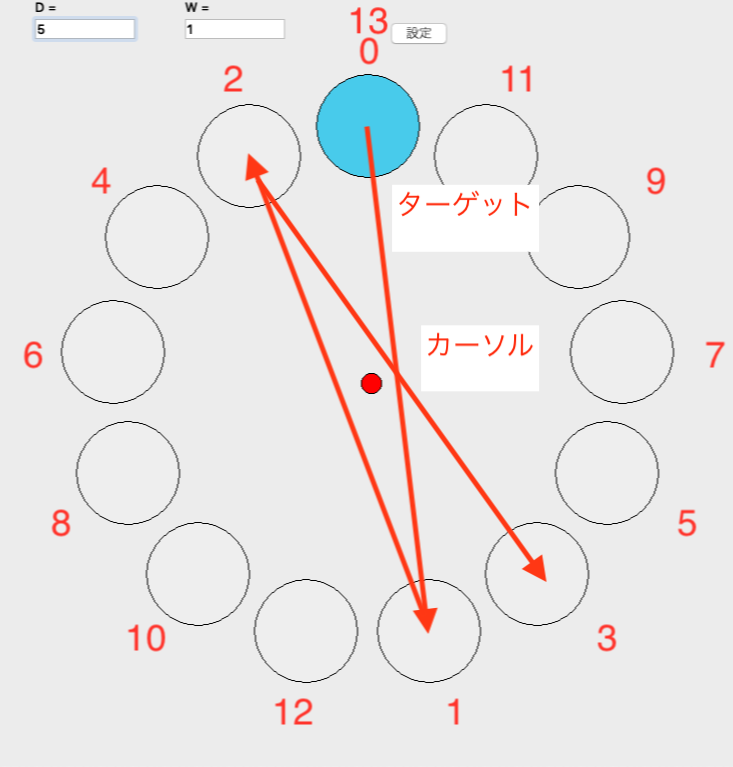
\includegraphics[angle = 270, width = 1.0\hsize]{./figures/mdpt.pdf}
	\end{center}
	\caption{実験において参加者が見る画面}
	\label{img:mdpt}
\end{figure}
\refImg{mdpt}は、実験プログラムの画面の一例であり、実験参加者はこの画面に従い操作を行う.
参加者は水色の円で示されるターゲットに,赤色の円で示されるカーソルを膝で操作し,2つが重なったときに選択操作を行う.
この選択操作1回を1試行と数える.
なお選択操作は足ではなくキーボード上のEnterキーで行う.
参加者は\refImg{mdpt}に示されている番号$0,1,...,13$の順にターゲットを選択する14試行を行う.ただし,$1,2,...,13$番の選択についてのみ実験データとして記録を行い,$0$番の選択は記録しない.\par
はじめ,ターゲットは全てオレンジ色で表示されている.
実験参加者がCommandキーを押すことで,実験が開始され,ターゲットを選択できるようになる.
13試行を終えると,再びターゲットはオレンジ色で表示される.
このとき,Shiftキーを押すことで,実験条件が変化する.
9条件すべてについて実験を行うことを1セッションと数える.
セッションの中で条件はランダムな順番で切り替わる.
実験は左膝,右膝について5セッションずつ行う.どちらかの膝について5セッション行うことを1ピリオドと数える.
解析のために,実験参加者が1回の試行に要した時間,選択おいてミスをしたかを表すフラグ,1試行における操作の開始点と終点およびターゲットとして表示されている円の中心座標を収集した.
参加者1人あたりのデータ数は,$13$(試行)$\times 9$(ターゲットサイズ条件)$\times 5$(セッション)$\times 2$(左右膝)$ = 1170$である.

参加者ははじめ椅子に座り,実験実施者が足の大腿と下腿の長さの計測を行う.下腿の長さは床から大腿の先端まで距離,大腿の長さは腰から大腿の先端までの距離とした.大腿,下腿の計測範囲を\refImg{leg_length}に示す.
\img{tb}{1.0}{leg_length.pdf}{大腿・下腿の計測範囲}{leg_length}

次に参加者はキャリブレーションを行い,上下左右の膝の可動範囲を記録する.
キャリブレーションの後,参加者は膝を移動させた方向にカーソルが追従するかを実験実施者と確認する.
追従に問題がある場合は再度キャリブレーションを行う.
問題がない場合,第1ピリオドを開始する.
第1ピリオドの終了後,5分間の休憩をとり,第2ピリオドを開始する.
第2ピリオドの終了後,後述するアンケートに回答する.



\subsection{評価方法}
評価にはフィッツの法則\cite{fitts}を用いる.
フィッツの法則は式\ref{eq:fitts}で表される.
\begin{eqnarray}
	MT_p = a + b\log_2{(D/W + 1)}
	\label{eq:fitts}
\end{eqnarray}
$MT_p$とはカーソルをターゲットに移動させるまでにかかると想定される時間である.
$a$と$b$は実験環境や機器に依存する定数である.
$D$はターゲット間の距離,$W$はターゲットの大きさ(円の直径)を表す.
なおこの実験では,$D$はターゲットが配置されている円周の直径としている.
また,$\log_2{(D/W + 1)}$という式はIndex of Difficulty($ID$)とも呼ばれ,課題の困難度を表す指標である.\par
$D$と$W$の大きさは以下の条件を用意した.
\begin{itemize}
	\item {D: } 3.0, 15.0, 26.0 \si{cm}
	\item {W: } 0.8, 1.8, 2.4 \si{cm}
\end{itemize}
これにより,9種類の$ID$ \{1.170, 1.415, 2.248, 2.858, 3.222, 3.565, 3.949, 4.304, 5.066\}を得る.\par
本研究における評価は,Soukoreffら\cite{Soukoreff:2004:TSP:1056153.1056155}によって示されている方法を参考にした.まず,それぞれの選択操作における$D_e$,$W_e$を$D$と$W$の大きさの組み合わせごとに次のように計算する.
\begin{enumerate}
	\item 選択操作1回ごとの始点と終点の間の直線距離$d$を計算する.始点は前回の選択操作においてEnterキーが押された位置,終点は今回の選択操作においてEnterキーが押された位置である.
	\item 選択操作1回ごとの終点と選択すべきターゲットの中心位置$w$との距離を計算する.
	\item $D_e$は$d$の平均,$W_e$は$w$の標準偏差である.
\end{enumerate}
求めた$D_e$,$W_e$から,ある$D$と$W$における$ID_e$は式\ref{eq:ide}で表される.
\begin{eqnarray}
	ID_e = \log_2{(D_e/W_e + 1)}
	\label{eq:ide}
\end{eqnarray}
次に,$ID$ごとに選択操作に要した時間の平均$MT$を求める.$MT$と$ID_e$から,線形回帰を用いて式\ref{eq:regression}における$a$,$b$を求める.
\begin{eqnarray}
	MT = a + b \times  ID_e
	\label{eq:regression}
\end{eqnarray}
また,左右の膝や,膝の移動方向における速度を比較するために,スループット$TP$を計算する.スループットは,式\ref{eq:tp}で求める.
\begin{eqnarray}
	TP = \cfrac{ID_e}{MT}
	\label{eq:tp}
\end{eqnarray}
式\ref{eq:regression}を用いて求めた線形回帰のグラフ,式\ref{eq:tp}を用いて求めたTP,および参加者ごとのエラー率から膝によるカーソル操作の性能評価を行う.さらにカーソルの移動方向が水平方向か垂直方向かで,性能が異なるかの調査を行う.\refImg{mdpt}において,水平方向の移動は選択ターゲットが6,7,8の時,垂直方向の移動は0,1,12,13の時と定義した.また,後述するアンケートから操作感や疲労感の評価を行う.

\subsection{実験機器}
実験に用いる機器は,ディスプレイ(DELL S2409Wb 24inch 1920$\times$ 1080),コンピュータ(Apple MacBookPro 2018 TouchBar),プロトタイプシステム,外付けキーボード(Apple Magic Keyboard 2)である.
$D$と$W$の大きさは,ディスプレイの実寸と解像度を元にプログラム内でピクセル値に変換されている.
%また,ノイズを軽減するため距離センサの真下に白いシートを敷いた.実験参加者は靴を脱いだ状態で足をシートに乗せて操作を行う.
\subsection{アンケート}
実験の最後に,参加者の疲労感と膝によるカーソル操作の難易の,2つの観点からアンケートを行った.
疲労感については以下の4項目を5点リッカート尺度で評価してもらった(1-全く疲れていない,5-とても疲れている).
\begin{itemize}
	\item {Q1: }太ももの疲労感
	\item {Q2: }ふくらはぎの疲労感
	\item {Q3: }足先の疲労感
	\item {Q4: }精神的な疲労感
\end{itemize}
加えて,項目になかった体の部位で疲れている箇所を自由記述形式で記述してもらった(Q5).
膝によるカーソル操作の難易については,以下の2項目を5点リッカート尺度で評価してもらった.
\begin{itemize}
	\item {Q6: }膝による操作は意図した通りに行うことができたか(1-全く行うことができなかった,5-とても行うことができた).
	\item {Q7: }膝を無理に動かさなければならない操作があったか(1-全く当てはまらなかった, 5-全て当てはまる).
\end{itemize}
加えて,膝による操作で簡単であった点,難しかった点を自由記述形式で記述してもらった(Q8).
\subsection{結果}
\subsubsection{カーソル操作の性能}
%エラー率
\refTb{errorrates}は左右の膝におけるターゲット選択のエラー率を,\refTb{errorrates_direction}は,その中から上下方向の移動のみ,左右方向の移動のみを抽出したときのエラー率を表している.全参加者のエラー率の平均は,左膝で$8.21\%$,右膝で$7.05\%$であった.
%\img{tb}{1.0}{errorrates.pdf}{選択操作のエラー率}{error_rate}
\begin{table}[tb]
	\begin{center}
		\begin{tabular}{|c|c|c|c|c|}
		\hline
 & 左膝 & 右膝 \\ \hline
P1 & 6.32\% & 5.64\% \\ \hline
P2 & 6.84\% & 5.13\% \\ \hline
P3 & 5.64\% & 7.86\% \\ \hline
P4 & 14.02\% & 9.57\% \\ \hline
平均 & 8.21\% & 7.05\% \\ \hline
		\end{tabular}
	\end{center}
	\caption{選択操作のエラー率(全体)}
	\label{tb:errorrates}
\end{table}
\begin{table}[tb]
	\begin{center}
		\begin{tabular}{|c|c|c|c|c|}
		\hline
  & \begin{tabular}{c} 左膝 \\ 垂直方向 \end{tabular} & \begin{tabular}{c} 左膝 \\ 水平方向 \end{tabular} & \begin{tabular}{c} 右膝 \\ 垂直方向 \end{tabular} & \begin{tabular}{c} 右膝 \\ 水平方向 \end{tabular} \\ \hline
P1 & 4.44\% & 8.15\% & 2.78\% & 8.15\% \\ \hline
P2 & 6.67\% & 3.70\% & 2.22\% & 7.41\% \\ \hline
P3 & 2.78\% & 7.41\% & 7.22\% & 10.37\% \\ \hline
P4 & 21.11\% & 12.59\% & 10.56\% & 8.89\% \\ \hline
平均 & 8.75\% & 7.96\% & 5.69\% & 8.70\% \\ \hline
		\end{tabular}
	\end{center}
	\caption{選択操作のエラー率(方向別)}
	\label{tb:errorrates_direction}
\end{table}

%生データグラフ
\refImg{regression_all}は,それぞれ左膝,右膝における実験結果である.また,\refImg{horizontal}は水平方向の移動,\refImg{vertical}は垂直方向の移動のみをそれぞれ取り出した実験結果である.縦軸が選択時間,横軸が実験結果から計算された$ID_e$を表す.各点は1試行の選択時間をそれぞれプロットしたものであり,参加者ごとに色と記号を分けている.また,各直線は参加者ごとの選択時間から,式\ref{eq:regression}によって線形回帰で求めた直線であり,参加者ごとに色を分けている.なお,点と直線の色は参加者ごとに対応する.

\img{tb}{1.0}{regression_all.pdf}{左右膝の選択時間と線形回帰モデル}{regression_all}
\img{tb}{1.0}{horizontal.pdf}{水平方向の移動に要した選択時間と線形回帰モデル}{horizontal}
\img{tb}{1.0}{vertical.pdf}{垂直方向の移動に要した選択時間と線形回帰モデル}{vertical}



%スループット
\refTb{tp}は,参加者ごとと全参加者の平均のスループットを表している.全参加者の平均のスループットは,左膝が$1.65$,右膝が$1.63$であった.この平均値について対応のあるt検定を行ったところ,有意差は認められなかった($t=0.14$,自由度:3).\par
\refTb{tp_direction}は垂直方向,水平方向のみの移動を抽出したものである.左膝における垂直方向の平均スループットは$1.78$,水平方向の平均スループットは$1.75$であった.この平均値について対応のあるt検定を行ったところ,有意差は認められなかった($t=0.20$,自由度:3).
右膝における垂直方向の平均スループットは$1.83$,水平方向の平均スループットは$1.65$であった.この平均値について不等分散を仮定したt検定を行ったところ,有意差は認められなかった($t=0.74$,自由度:6).
\begin{table}[tb]
	\begin{center}
		\begin{tabular}{|c|c|c|c|c|}
		\hline
 & 左膝 & 右膝 \\ \hline
P1 & 1.54  & 1.55  \\ \hline
P2 & 2.04  & 1.90  \\ \hline
P3 & 1.66  & 1.37  \\ \hline
P4 & 1.37  & 1.71  \\ \hline
平均 & 1.65  & 1.63  \\ \hline
		\end{tabular}
	\end{center}
	\caption{スループット(全体)}
	\label{tb:tp}
\end{table}
\begin{table}[tb]
	\begin{center}
		\begin{tabular}{|c|c|c|c|c|}
		\hline
  & \begin{tabular}{c} 左膝 \\ 垂直方向 \end{tabular} & \begin{tabular}{c} 左膝 \\ 水平方向 \end{tabular} & \begin{tabular}{c} 右膝 \\ 垂直方向 \end{tabular} & \begin{tabular}{c} 右膝 \\ 水平方向 \end{tabular} \\ \hline
P1 & 1.67  & 1.56  & 1.79  & 1.49  \\ \hline
P2 & 2.34  & 2.00  & 2.26  & 2.08  \\ \hline
P3 & 1.86  & 1.81  & 1.47  & 1.26  \\ \hline
P4 & 1.24  & 1.61  & 1.81  & 1.79  \\ \hline
平均 & 1.78  & 1.75  & 1.83  & 1.65  \\ \hline
		\end{tabular}
	\end{center}
	\caption{スループット(方向別)}
	\label{tb:tp_direction}
\end{table}

%\img{tb}{0.85}{throughput.pdf}{左右膝のスループット}{tp}


\subsubsection{アンケート結果}
%\img{tb}{1.0}{enquette.pdf}{Q1,2,3,4,6,7のアンケート結果}{enquette}
\begin{table}[tb]
	\begin{center}
		\begin{tabular}{|c|c|c|c|c|c|c|}
		\hline
 & Q1 & Q2 & Q3 & Q4 & Q6 & Q7 \\ \hline
P1 & 4 & 4 & 2 & 2 & 5 & 1 \\ \hline
P2 & 4 & 2 & 3 & 3 & 4 & 2 \\ \hline
P3 & 1 & 2 & 1 & 2 & 4 & 1 \\ \hline
P4 & 4 & 4 & 3 & 3 & 4 & 1 \\ \hline
平均 & 3.25 & 3.00 & 2.25 & 2.50 & 4.25 & 1.25 \\ \hline
		\end{tabular}
	\end{center}
	\caption{アンケート結果(Q1,Q2,Q3,Q4,Q6,Q7)}
	\label{tb:enquette}
\end{table}
\refTb{enquette}はアンケートの中で,リッカート尺度で評価を行った,Q1,Q2,Q3,Q4,Q6,Q7における結果である.疲労感について質問したQ4において,Q1では4人中3人の参加者が4(=疲れている)と回答している.しかし操作感について質問したQ6,Q7において,すべての参加者がQ6では4(=意図した通りに操作を行うことができた)または5(=とても意図した通りに操作を行うことができた)と回答し,Q7では1(=膝を無理に動かさなければいけない操作は全く当てはまらない)または2(=膝を無理に動かさなければいけない操作はあまり当てはまらない)と回答している.\par
また自由記述での回答を求めたQ5,Q8では,
Q5においては,目(P1)に疲労感を感じたという意見を受けた.これは,1ピリオドあたり20〜25分間の長い間,画面を見続けたことが原因であると考える.また,Q8においては,引くとき(下方向の膝の移動)の摩擦が少し重い(P1),細かい修正が難しかった(P3)という意見があった.

\subsection{考察}
左右の膝におけるスループットの値は,数値のみの比較では,Vellosoら\cite{velloso:hal-01599657}による足先を用いたカーソル操作の結果(左足:$1.16$,右足:$1.14$)より高いものである.一方でHorodniczyら\cite{Horodniczy:2017:FHE:3025453.3025625}による足先を用いながらも補助装置を取り付けた手法(右足のみ:$2.21$)と比較すると低い.したがって,膝によるカーソル操作は足による操作より高速に行える可能性があるが,膝の移動方向やシステムの設計など,改良の余地があると考える.\par
またエラー率に関してはVellosoら\cite{velloso:hal-01599657}の結果とほぼ同等であるといえる.しかし,他の参加者と比べると、P4のエラー率が高い結果となっている.データでは、\refTb{length}を見ても、参加者間で足の長さにほとんど差はないが,$W$に対して$W_e$が最大で3倍程度大きくなっている条件が存在した.これらの結果から,2つの原因があると考える.1つ目に、P4は他の参加者よりカーソルとターゲットとのずれを大きく許容していた可能性がある。2つ目に、Enterキーを押す瞬間に、膝と距離センサとの距離が、計測できる範囲より小さくなってしまった可能性がある。この場合距離センサの仕様上、膝との距離が一番小さいはずの距離センサは計測できる距離の最大値を出力してしまう。$K^t_y$が距離データの中の最小の距離から計算されるのに対し、$K^t_x$は各距離センサに対して、膝との距離を重み付けして計算される。したがって、最終的なカーソル座標$P^t_x$が瞬間的に大きく変化してしまったと考える。
%これは,キャリブレーション時に上下の膝位置の差が小さく,小さな膝の動きに対してカーソルの移動量が大きくなってしまったことが考えられる.
%今後プロトタイプシステムの膝位置認識や座標計算の方法を見直すことで改善を図る.\par
%移動方向別の分析では,スループットの面で水平方向よりも垂直方向の方が高い値を示した一方で,アンケートでは下方向の移動が難しいという意見が多かった.これは,左右方向の膝位置認識では全ての距離センサから送信されるデータを総合しているのに対し,上下方向には距離センサの最小値が膝位置となるので,より正確な位置となっていると考える.\par
アンケートからは,太ももやふくらはぎには疲労が溜まりやすい一方で,操作は意図した通り,無理な動きも少なく行えたと読み取れる.今後疲労感を軽減できるような膝の入力方法が必要と考える.

%\section{応用例:一人称視点ゲームにおける膝によるプレイヤー移動}
%本プロトタイプシステムの応用例として,一人称視点ゲームのプレイヤーを,膝を用いて前後左右に移動させることを提案する.PC上でプレイする一人称視点ゲームでは,一般にマウスを前後左右に動かすことで視点を上下左右に,キーボードでプレイヤーの移動方向を操作する.しかしキーボードとマウスを常に同時に操作するために,机上に大きなスペースが必要になるといった問題がある.プレイヤーの移動を膝で代用することにより,こうした問題を解決できるのではないかと考える.
%我々は,Unityを用いて\refImg{}のようなサンプルプログラムを実装した.膝の位置を認識し,片方の膝を上下左右に操作した時にプレイヤーが前後左右に移動するスクリプトを実装し,プレイヤーの移動を実現した.

\section{今後の展望・課題}
本プロトタイプシステムは片膝のみでの使用を想定しているが,両膝で使用できるようになれば更なる入力の拡張も考えられる.これは,2つの距離センサを使うことで実現できる.しかし,スカートや膝掛けなど,両膝が衣服によって接続されている場合には正しく膝の位置を認識することはできない.これには使用するセンサを変更するなどの必要があると考えている.\par
本研究では膝単体を用いてカーソル操作を行った.今後手による入力と組み合わせることで更なるインタラクションが実現できる.例えば,マウスでファイルを選択した状態で,膝でファイルを動かすことができれば,マウスの移動量を減らすことができ,小さい机でも快適にマウスを使用できる.\par

\section{結論}
本研究では膝による入力を実現する第一歩として,机の裏に設置した距離センサアレイによって膝の位置を認識し,カーソル操作を行ったときの性能を調査した.
また距離センサアレイは特別な装置を足に取り付ける必要がなく,装置がユーザの邪魔となりにくい.
我々は距離センサアレイから距離データを取得し,膝の位置を認識し,カーソル座標へ変換するプロトタイプシステムを実装した.
プロトタイプシステムを用いた実験では,膝によるカーソル操作は足による操作より高速に行える可能性があり,操作は意図した通り無理なく行えるという結果を得た
%さらに,VR一人称視点ゲームへの膝による操作の応用例の提案を行った.
今後は,ユーザが様々な衣服を着用した場合の対応や,手を中心とした他の入力モダリティとの組み合わせを探索する.


%% bib
\bibliographystyle{ipsjunsrt-e}
%\bibliographystyle{ipsjsort}
%\bibliographystyle{junsrt}
%\bibliography{bibsample}
\bibliography{ref.bib}



\begin{biography}
\profile{m,E}{情報 太郎}{1970年生.1992年情報処理大学理学部情報科学科卒業.
1994年同大学大学院修士課程修了.同年情報処理学会入社.オンライン出版の研究
に従事.電子情報通信学会,IEEE,ACM 各会員.}
%
\profile{n}{処理 花子}{1960年生.1982年情報処理大学理学部情報科学科卒業.
1984年同大学大学院修士課程修了.1987年同博士課程修了.理学博士.1987年情報処
理大学助手.1992年架空大学助教授.1997年同大教授.オンライン出版の研究
に従事.2010年情報処理記念賞受賞.電子情報通信学会,IEEE,IEEE-CS,ACM
各会員.}
%
\profile{h,L}{学会 次郎}{1950年生.1974年架空大学大学院修士課程修了.
1987年同博士課程修了.工学博士.1977年架空大学助手.1992年情報処理大学助
教授.1987年同大教授.2000年から情報処理学会顧問.オンライン出版の研究
に従事.2010年情報処理記念賞受賞.情報処理学会理事.電子情報通信学会,
IEEE,IEEE-CS,ACM 各会員.}
\end{biography}



\end{document}
